\documentclass[pdf,aspectratio=169]{beamer}
\usepackage[]{hyperref,graphicx,siunitx,lmodern,booktabs}
\usepackage{physics}
\usepackage{em-commands}
\mode<presentation>{\usetheme{EM}}

%Question Numbering
\newcounter{questionnumber}
\newcommand{\qnum}{%
	\stepcounter{questionnumber}%
	Q\arabic{questionnumber}
}
\resetcounteronoverlays{questionnumber}

\graphicspath{ {../Images/} }

\sisetup{per-mode=symbol}

%preamble
\title{Separating the X's from the Y's}
\date{October 1, 2018}
\author{Jed Rembold}

\begin{document}
\renewcommand{\theenumi}{\Alph{enumi}}

\begin{frame}{Announcements}
	\begin{itemize}
		\item Homework 5 due tonight!
			\begin{itemize}
				\item Take a look over comments from the graded HW4 to make sure you aren't forgetting anything on your plots!
			\end{itemize}
		\item Those test polling results\ldots
		\item Have read Ch 3.3.2 by Wednesday
	\end{itemize}
\end{frame}

\begin{frame}{\qnum}
	Say you have three functions $f(x)$, $g(y)$, and $h(z)$. Each function only depends on it's single variable, and not on the others. If
	\[f(x) + g(y) + h(z) = 0\]
	for all $x,y,z$, then:
	\begin{enumerate}
		\item \alert<2>{All three functions must be constant (i.e.\ they do not depend on $x,y,z$ at all)}
		\item At least one of the functions must be equal to 0 everywhere
		\item All of the functions must be equal to zero everywhere
		\item All three functions must be linear (e.g.\ $f(x) = ax +b,\,\, g(y) = cy + d$ etc.)
	\end{enumerate}
\end{frame}

\begin{frame}{\qnum}
	Say our general solutions contains the expression:
	\[X(x) = Ae^{\sqrt{c}x} + Be^{-\sqrt{c}x}\]
	What does our solution look like if $c < 0$? What about if $c > 0$?
	\begin{enumerate}
		\item Exponential, and Sinusoidal
		\item \alert<2>{Sinusoidal, and Exponential}
		\item Both Exponential
		\item Both Sinusoidal
	\end{enumerate}
\end{frame}

\begin{frame}{\qnum}
	Given the two differential equations:
	\[\frac{1}{X}\dv[2]{X}{x} = C_1 \qand \frac{1}{Y}\dv[2]{Y}{y} = C_2\]
	where $C_1 + C_2 = 0$. Given the boundary conditions in the below figure, which coordinate should be assigned to the negative constant?
	\begin{columns}
		\column{0.5\textwidth}
		\begin{enumerate}
			\item $x$
			\item \alert<2>{$y$}
			\item $C_1 =C_2 = 0$ here
			\item It doesn't matter
		\end{enumerate}
		\column{0.5\textwidth}
		\begin{center}
			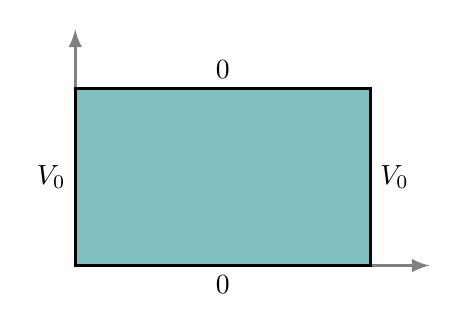
\begin{tikzpicture}[scale=1.5]
				\path[help lines,very thick, -latex] (0,0) edge +(0,2) (0,0) edge +(3,0);
				\draw[very thick, fill=Teal!50] (0,0) rectangle +(2.5, 1.5);
				\node[left] at (0,.75) {$V_0$};
				\node[right] at (2.5,.75) {$V_0$};
				\node[below] at (1.25,0) {0};
				\node[above] at (1.25,1.5) {0};
			\end{tikzpicture}
		\end{center}
	\end{columns}
\end{frame}

\begin{frame}{\qnum}
	Given the two differential equations:
	\[\frac{1}{X}\dv[2]{X}{x} = C_1 \qand \frac{1}{Y}\dv[2]{Y}{y} = C_2\]
	where $C_1 + C_2 = 0$. Given the boundary conditions in the below figure, which coordinate should be assigned to the negative constant?
	\begin{columns}
		\column{0.5\textwidth}
		\begin{enumerate}
			\item $x$
			\item $y$
			\item $C_1 =C_2 = 0$ here
			\item \alert<2>{It doesn't matter}
		\end{enumerate}
		\column{0.5\textwidth}
		\begin{center}
			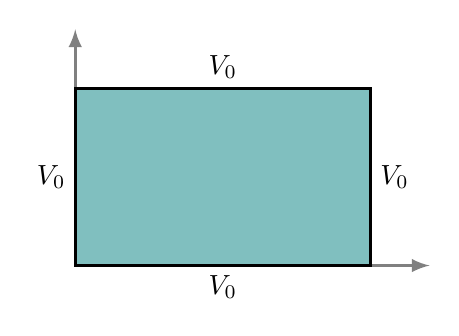
\begin{tikzpicture}[scale=1.5]
				\path[help lines,very thick, -latex] (0,0) edge +(0,2) (0,0) edge +(3,0);
				\draw[very thick, fill=Teal!50] (0,0) rectangle +(2.5, 1.5);
				\node[left] at (0,.75) {$V_0$};
				\node[right] at (2.5,.75) {$V_0$};
				\node[below] at (1.25,0) {$V_0$};
				\node[above] at (1.25,1.5) {$V_0$};
			\end{tikzpicture}
		\end{center}
	\end{columns}
\end{frame}

\begin{frame}{\qnum}
	When would the boundary condition
	\[V(x,a) = Ce^{-kx}\cos(ky) = 0\]
	tell you?
	\begin{enumerate}
		\item It must be that $k=0$
		\item \alert<2>{It must be that $\displaystyle k = \frac{n\pi}{2a}$}
		\item It must be that $\displaystyle k=\frac{n\pi}{a}$
		\item It must be that $C=0$
	\end{enumerate}
\end{frame}

\begin{frame}{\qnum}
	What is the result of
	\[\int_0^{2\pi}\sin(2x)\sin(3x)\,dx\]
	\begin{enumerate}
		\item \alert<2>{0}
		\item $\pi$
		\item $2\pi$
		\item Give me another second, consulting Sympy\ldots
	\end{enumerate}
\end{frame}

\begin{frame}{\qnum}
	Why does Fourier's trick work to find the values of $C_n$?
	\begin{enumerate}
		\item Because the infinite sum of sine waves always approaches a constant
		\item Because any function can be expressed as a sum of different sine waves
		\item Because sine functions are orthogonal to one another
		\item \alert<2>{C and B}
	\end{enumerate}
\end{frame}


\end{document}
